\documentclass[a4paper]{book}\usepackage[]{graphicx}\usepackage[]{color}
%% maxwidth is the original width if it is less than linewidth
%% otherwise use linewidth (to make sure the graphics do not exceed the margin)
\makeatletter
\def\maxwidth{ %
  \ifdim\Gin@nat@width>\linewidth
    \linewidth
  \else
    \Gin@nat@width
  \fi
}
\makeatother

\definecolor{fgcolor}{rgb}{0.345, 0.345, 0.345}
\newcommand{\hlnum}[1]{\textcolor[rgb]{0.686,0.059,0.569}{#1}}%
\newcommand{\hlstr}[1]{\textcolor[rgb]{0.192,0.494,0.8}{#1}}%
\newcommand{\hlcom}[1]{\textcolor[rgb]{0.678,0.584,0.686}{\textit{#1}}}%
\newcommand{\hlopt}[1]{\textcolor[rgb]{0,0,0}{#1}}%
\newcommand{\hlstd}[1]{\textcolor[rgb]{0.345,0.345,0.345}{#1}}%
\newcommand{\hlkwa}[1]{\textcolor[rgb]{0.161,0.373,0.58}{\textbf{#1}}}%
\newcommand{\hlkwb}[1]{\textcolor[rgb]{0.69,0.353,0.396}{#1}}%
\newcommand{\hlkwc}[1]{\textcolor[rgb]{0.333,0.667,0.333}{#1}}%
\newcommand{\hlkwd}[1]{\textcolor[rgb]{0.737,0.353,0.396}{\textbf{#1}}}%

\usepackage{framed}
\makeatletter
\newenvironment{kframe}{%
 \def\at@end@of@kframe{}%
 \ifinner\ifhmode%
  \def\at@end@of@kframe{\end{minipage}}%
  \begin{minipage}{\columnwidth}%
 \fi\fi%
 \def\FrameCommand##1{\hskip\@totalleftmargin \hskip-\fboxsep
 \colorbox{shadecolor}{##1}\hskip-\fboxsep
     % There is no \\@totalrightmargin, so:
     \hskip-\linewidth \hskip-\@totalleftmargin \hskip\columnwidth}%
 \MakeFramed {\advance\hsize-\width
   \@totalleftmargin\z@ \linewidth\hsize
   \@setminipage}}%
 {\par\unskip\endMakeFramed%
 \at@end@of@kframe}
\makeatother

\definecolor{shadecolor}{rgb}{.97, .97, .97}
\definecolor{messagecolor}{rgb}{0, 0, 0}
\definecolor{warningcolor}{rgb}{1, 0, 1}
\definecolor{errorcolor}{rgb}{1, 0, 0}
\newenvironment{knitrout}{}{} % an empty environment to be redefined in TeX

\usepackage{alltt}
\usepackage[utf8]{inputenc}
\usepackage{amsmath}
\usepackage[french]{babel}
\usepackage[T1]{fontenc}
\usepackage{amsfonts}
\usepackage{amssymb}
\usepackage{xcolor}
\usepackage{hyperref}
\usepackage{tikz}
\usepackage{fancyvrb}
\usepackage{booktabs}
\usepackage{graphicx}
\usepackage{pgfsys}
\usepackage{keyval}
\usepackage{subfig}
\usepackage{multicol}
% \usepackage{placeins} % gestion des flottants

\voffset -2cm
\hoffset 0cm
\oddsidemargin 0cm
\evensidemargin -0.5cm
\textwidth 17cm
\topmargin 1cm
\textheight 24cm
\parindent 0cm
\columnsep 0.7cm

%%%%%%%%%%%%%%%%%%%%%%%%%%%%%%













%%%%%%%%%%%%%%%%%%%%%%%%%%%%%%
\IfFileExists{upquote.sty}{\usepackage{upquote}}{}
\begin{document}
\thispagestyle{empty} % la page en tour n'a pas de numéro de page

\begin{multicols}{2}

\includegraphics[height=2cm]{Images/logo.png}
\begin{flushright}

\includegraphics[height=2cm]{Images/logoONF.png}
\end{flushright}

\end{multicols}

\vspace*{3cm}
\begin{center}
\textbf{SUIVI DENDROMÉTRIQUE DES ESPACES PROTÉGÉS}
% \date{\today}

\end{center}

\begin{center}
Dispositif n°2 : RN Frankenthal
\end{center}

\vspace*{2cm}
\begin{center}
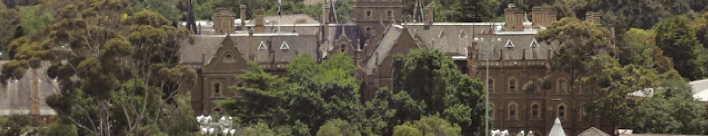
\includegraphics[width=15cm]{Images/RB2.png}
\end{center}

\vspace*{1cm}
\begin{center}
\today
\end{center}

% \clearpage
\tableofcontents
\thispagestyle{empty} % la page en tour n'a pas de numéro de page
\setcounter{page}{0}


\chapter{Présentation du site}

\section{Généralités}

\subsection{Renseignements administratifs}

\begin{tabular}{ll}
Nom : & RN Frankenthal \\
Commune(s): & \\
Département(s): & \\
Région(s): & \\
Pays : & France\\

\end{tabular}

% latex table generated in R 3.1.2 by xtable 1.7-4 package
% Mon Nov 24 09:52:02 2014
\begin{table}[ht]
\centering
{\footnotesize
\begin{tabular}{rl}
  \hline
 & Statut1 \\ 
  \hline
Code INPN & FR3600126 \\ 
  Surface & 746.36 \\ 
  Date création &  \\ 
   \hline
\end{tabular}
}
\caption{Statuts de protection.} 
\label{Statuts}
\end{table}



\subsection{Contacts}
\begin{tabular}{ll}
Organisme : & \\
Gestionnaire : & \\
Nom : & \\
Prénom : & \\
Adresse : & \\
  & \\
Tel. : & \\
Email : & \\
\end{tabular}

\newpage
\subsection{Carte de localisation}
La carte située en figure \ref{fig:PlanLoc} présente la réserve sur un fond Google.

\begin{knitrout}
\definecolor{shadecolor}{rgb}{0.969, 0.969, 0.969}\color{fgcolor}\begin{figure}[H]


{\centering 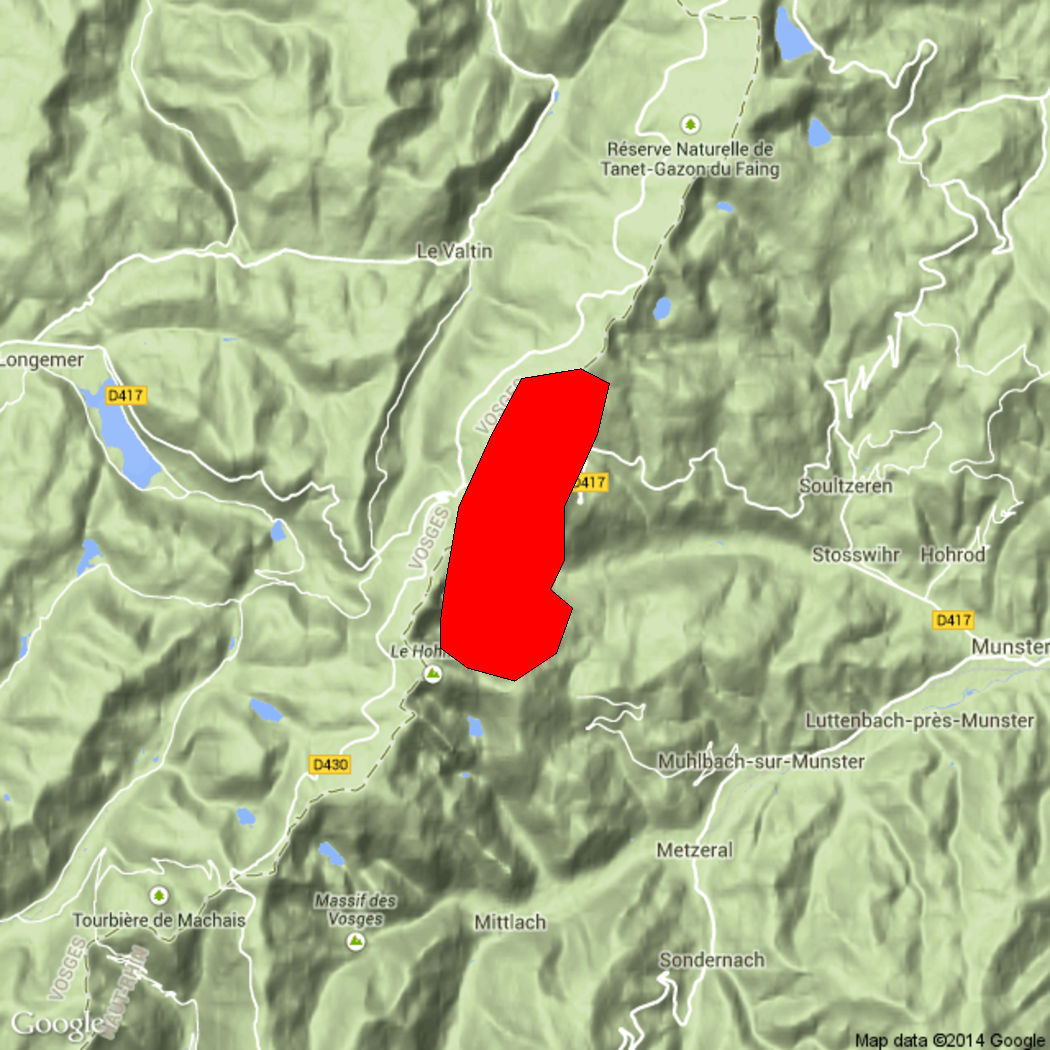
\includegraphics[width=.7\linewidth,scale=1]{Figures/PlanLoc-1} 

}

\caption[Localisation de la réserve]{Localisation de la réserve\label{fig:PlanLoc}}
\end{figure}


\end{knitrout}



\subsection{Milieux}

La figure \ref{fig:CarteSER} fournit la localisation de la réserve dans sa sylvoécorégion.

\begin{knitrout}
\definecolor{shadecolor}{rgb}{0.969, 0.969, 0.969}\color{fgcolor}\begin{figure}[h]


{\centering 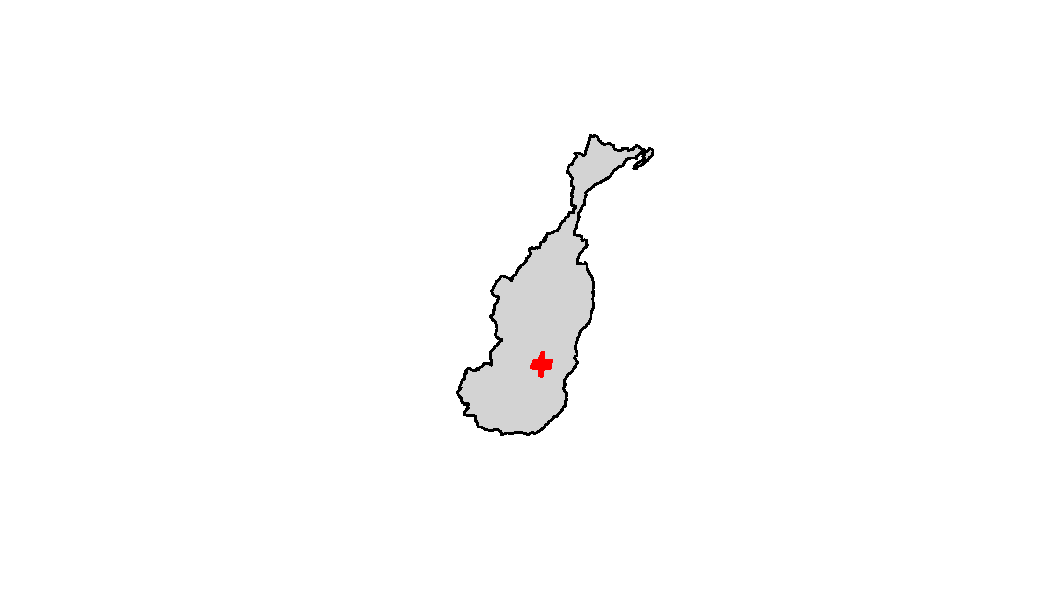
\includegraphics[width=\maxwidth]{Figures/CarteSER-1} 

}

\caption[Localisation de la réserve dans sa sylvoécorégion]{Localisation de la réserve dans sa sylvoécorégion.\label{fig:CarteSER}}
\end{figure}


\end{knitrout}


\begin{tabular}{ll}
Habitats : & \\
GRECO : & \\
Sylvoécorégions : & Massif vosgien central\\
Altitude min : &  \\
Altitude max : &  \\
\end{tabular} \\



\subsection{Echantillonnage}
\subsubsection{Stratégie}
Installé en 2009, le dispositif a fait l’objet de 1 cycle(s) de mesure.\\

La réserve a été divisée en strates. Le tableau \ref{Echantillonnage} résume les principaux paramètres de l'échantillonnage. \\
% latex table generated in R 3.1.2 by xtable 1.7-4 package
% Mon Nov 24 09:52:02 2014
\begin{table}[ht]
\centering
{\footnotesize
\begin{tabular}{rl}
  \hline
 & Strate1 \\ 
  \hline
Nom/raison &  \\ 
  Surface &  \\ 
  Nombre de placettes & 115 \\ 
  Nombre d’arbres & 3235 \\ 
  Nombre moyen d’arbres par placette & 28.1 \\ 
  Densité du maillage &  \\ 
  Angle relascopique & 3 (115) \\ 
  Diamètre de précomptage pour l'angle fixe &  \\ 
   \hline
\end{tabular}
}
\caption{Principaux paramètres de l'échantillonnage par strate.} 
\label{Echantillonnage}
\end{table}


\subsubsection{Nombre d'individus échantillonnés}

\begin{center}
  \begin{tabular}{rl}
$3235$     & arbres vivants \\
$1280$        & arbres morts sur pied \\
$521$   & billons au sol de diam sup à 30 cm\\
$510$    & billons au sol de diam inf à 30 cm\\
$154$       & relevés de régénération \\
  \end{tabular}
\end{center}


La figure \ref{fig:DiamDist} située en annexe permet de vérifier si l'échantillon est en accord avec le protocole. Elle permet  de détecter les arbres limites. \\

Le tableau \ref{Tarifs} également situé en annexe rappelle les tarifs de cubage retenus par l'opérateur. Le tableau XXX fournit quand à lui le tarif de cubage volume géométrique bois fort tige obtenu à partir de la base de données de l'IFN.


\section{Tableaux de synthèse}
\subsection{Arbres vivants}
Le tableau \ref{Dendro} fournit les principales caractéristiques dendrométriques (volume, surface terrière et nombre de tiges à l'hectare) des arbres vivants, accompagnées de leur coefficient de variation et précision. \\

% latex table generated in R 3.1.2 by xtable 1.7-4 package
% Mon Nov 24 09:52:02 2014
\begin{table}[ht]
\centering
{\footnotesize
\begin{tabular}{rrrrrrrrrrrr}
  \hline
 & Cycle & Vha & Gha & Nha & Vha\_cv & Gha\_cv & Nha\_cv & Vha\_er & Gha\_er & Nha\_er & Nbre \\ 
  \hline
12 & 1 & 453 & 38.2 & 692 & 41.9 & 40.1 & 66.3 & 7.7 & 7.4 & 12.2 & 115 \\ 
   \hline
\end{tabular}
}
\caption{Principales caratéristiques dendrométriques, ainsi que leur précision.} 
\label{Dendro}
\end{table}


La figure \ref{fig:GraphDendro} complète le tableau \ref{Dendro} en illustrant la variabilité des données. \\
\begin{knitrout}\footnotesize
\definecolor{shadecolor}{rgb}{0.969, 0.969, 0.969}\color{fgcolor}\begin{figure}[H]


{\centering 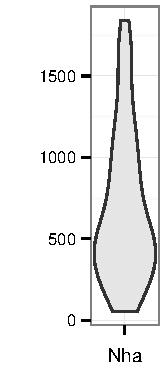
\includegraphics[width=\maxwidth]{Figures/GraphDendro-1} 
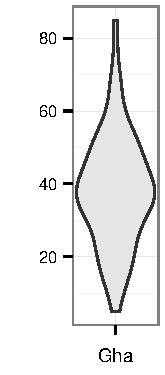
\includegraphics[width=\maxwidth]{Figures/GraphDendro-2} 
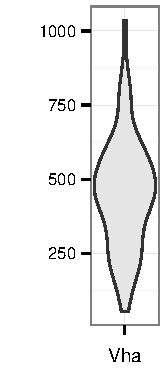
\includegraphics[width=\maxwidth]{Figures/GraphDendro-3} 

}

\caption[Variabilité des principales caractéristiques dendrométriques]{Variabilité des principales caractéristiques dendrométriques\label{fig:GraphDendro}}
\end{figure}


\end{knitrout}


Le tableau \ref{Structure} fournit la répartition des principales caractéristiques dendrométriques (volume, surface terrière et nombre de tiges à l'hectare) des arbres vivants par catégories de diamètre, accompagnée de leur coefficient de variation et précision.

% latex table generated in R 3.1.2 by xtable 1.7-4 package
% Mon Nov 24 09:52:03 2014
\begin{table}[ht]
\centering
{\footnotesize
\begin{tabular}{rlrrrrrrrrr}
  \hline
Cycle & Cat & MoyVha & MoyGha & MoyNha & CVVha & CVGha & CVNha & ErVha & ErGha & ErNha \\ 
  \hline
1 & PER & 34 & 3.9 & 307 & 108.0 & 108.2 & 111.7 & 20.0 & 20.0 & 20.6 \\ 
  1 & PB & 84 & 7.7 & 198 & 93.6 & 93.4 & 93.2 & 17.3 & 17.2 & 17.2 \\ 
  1 & BM & 172 & 14.2 & 144 & 76.1 & 75.9 & 78.2 & 14.0 & 14.0 & 14.5 \\ 
  1 & GB & 107 & 8.3 & 35 & 98.0 & 97.9 & 97.5 & 18.1 & 18.1 & 18.0 \\ 
  1 & TGB & 55 & 4.2 & 9 & 135.9 & 135.3 & 129.0 & 25.1 & 25.0 & 23.8 \\ 
   \hline
\end{tabular}
}
\caption{Analyse de la structure des peuplements. Valeurs moyennes et précisions associées à l'échelle de la réserve.} 
\label{Structure}
\end{table}


\subsection{Bois morts}
Le tableau \ref{BoisMort} fournit l'importance globale du bois mort, ainsi que sa répartition en 4 grandes classes. Les moyennes sont accompagnées de leur précision. La légende du tableau est la suivante : \\
VSinf = volume au sol inférieur à 30cm, \\
VSsup = volume au sol supérieur à 30cm, \\
VPinf = volume sur pied inférieur à 30cm, \\
VPsup = volume sur pied supérieur à 30cm \\

% latex table generated in R 3.1.2 by xtable 1.7-4 package
% Mon Nov 24 09:52:03 2014
\begin{table}[ht]
\centering
{\footnotesize
\begin{tabular}{rrrrrrrrrrr}
  \hline
Cycle & VSinf & VSsup & VPinf & VPsup & VT & VSinf\_er & VSsup\_er & VPinf\_er & VPsup\_er & VT\_er \\ 
  \hline
1 & 3.9 & 35.8 & 13.4 & 19.3 & 72.5 & 28.3 & 28.0 & 19.6 & 27.7 & 18.7 \\ 
   \hline
\end{tabular}
}
\caption{Importance et type de bois mort.} 
\label{BoisMort}
\end{table}


La figure \ref{fig:GraphBMT} complète le tableau \ref{BoisMort} en illustrant la variabilité des données.
\begin{knitrout}\footnotesize
\definecolor{shadecolor}{rgb}{0.969, 0.969, 0.969}\color{fgcolor}\begin{figure}[H]


{\centering 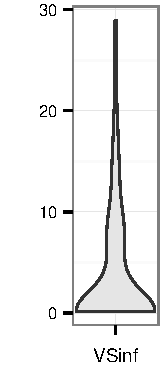
\includegraphics[width=\maxwidth]{Figures/GraphBMT-1} 
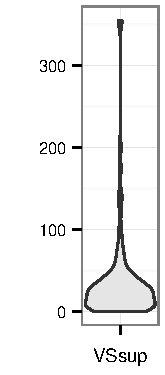
\includegraphics[width=\maxwidth]{Figures/GraphBMT-2} 
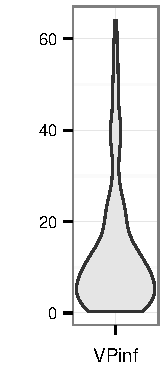
\includegraphics[width=\maxwidth]{Figures/GraphBMT-3} 
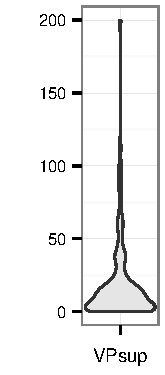
\includegraphics[width=\maxwidth]{Figures/GraphBMT-4} 
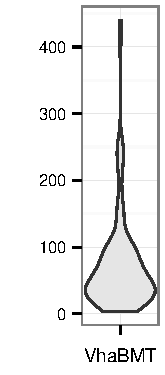
\includegraphics[width=\maxwidth]{Figures/GraphBMT-5} 

}

\caption[Variabilité des types de bois mort]{Variabilité des types de bois mort\label{fig:GraphBMT}}
\end{figure}


\end{knitrout}

\section{Cartes thématiques}


\subsection{Localisation des placettes}

\subsection{Bois vivant}
La figure \ref{fig:CartePlacettes} permet de localiser les placettes au sein du périmètre de la réserve. Elle fournit également la répartition du volume à l'hectare
\begin{knitrout}
\definecolor{shadecolor}{rgb}{0.969, 0.969, 0.969}\color{fgcolor}\begin{figure}[h]


{\centering 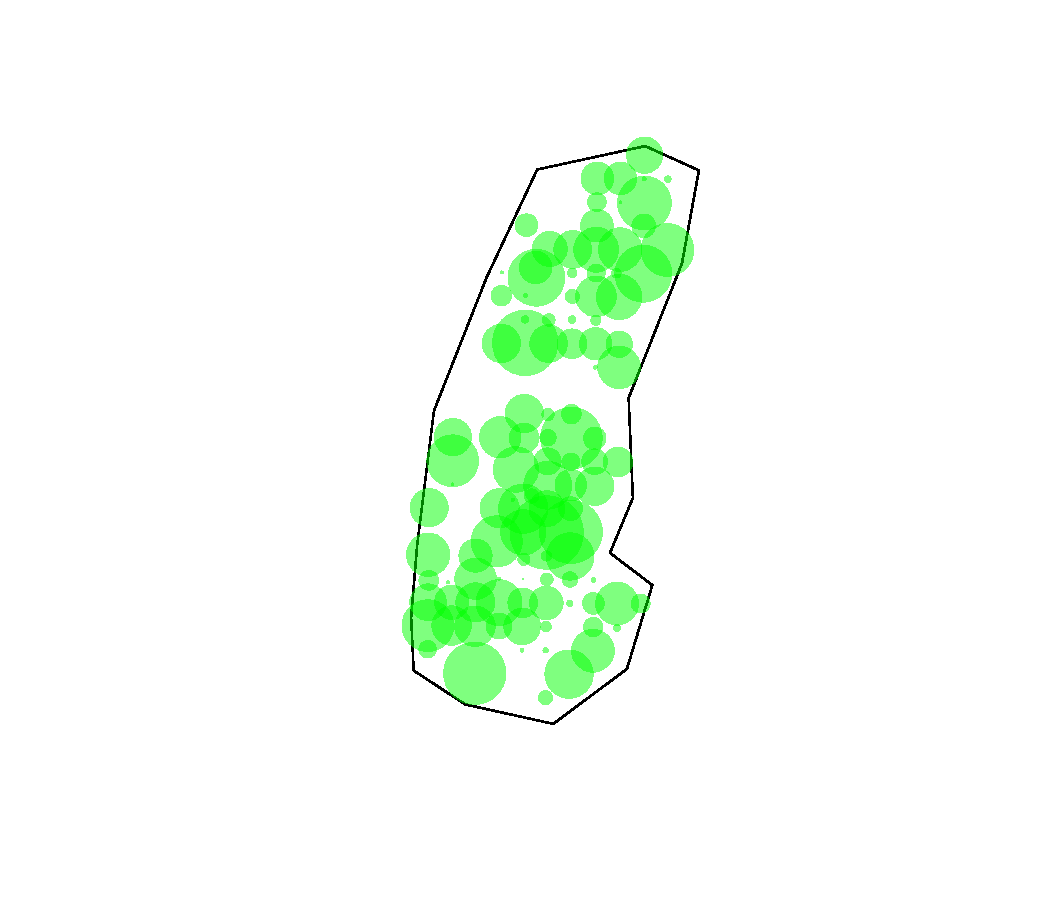
\includegraphics[width=\maxwidth]{Figures/CartePlacettes-1} 

}

\caption[Périmètre et localisation des placettes]{Périmètre et localisation des placettes. Répartition du volume à l'hectare.\label{fig:CartePlacettes}}
\end{figure}


\end{knitrout}


\subsection{Bois mort}
La figure \ref{fig:CarteVolBMS} permet de visualiser la répartition du bois mort au sol. La figure \ref{fig:CarteVolBMP} permet de visualiser la répartition du bois mort sur pied.

\begin{knitrout}
\definecolor{shadecolor}{rgb}{0.969, 0.969, 0.969}\color{fgcolor}\begin{figure}[H]
\subfloat[inf à 30 cm\label{fig:CarteVolBMS1}]{

{\centering 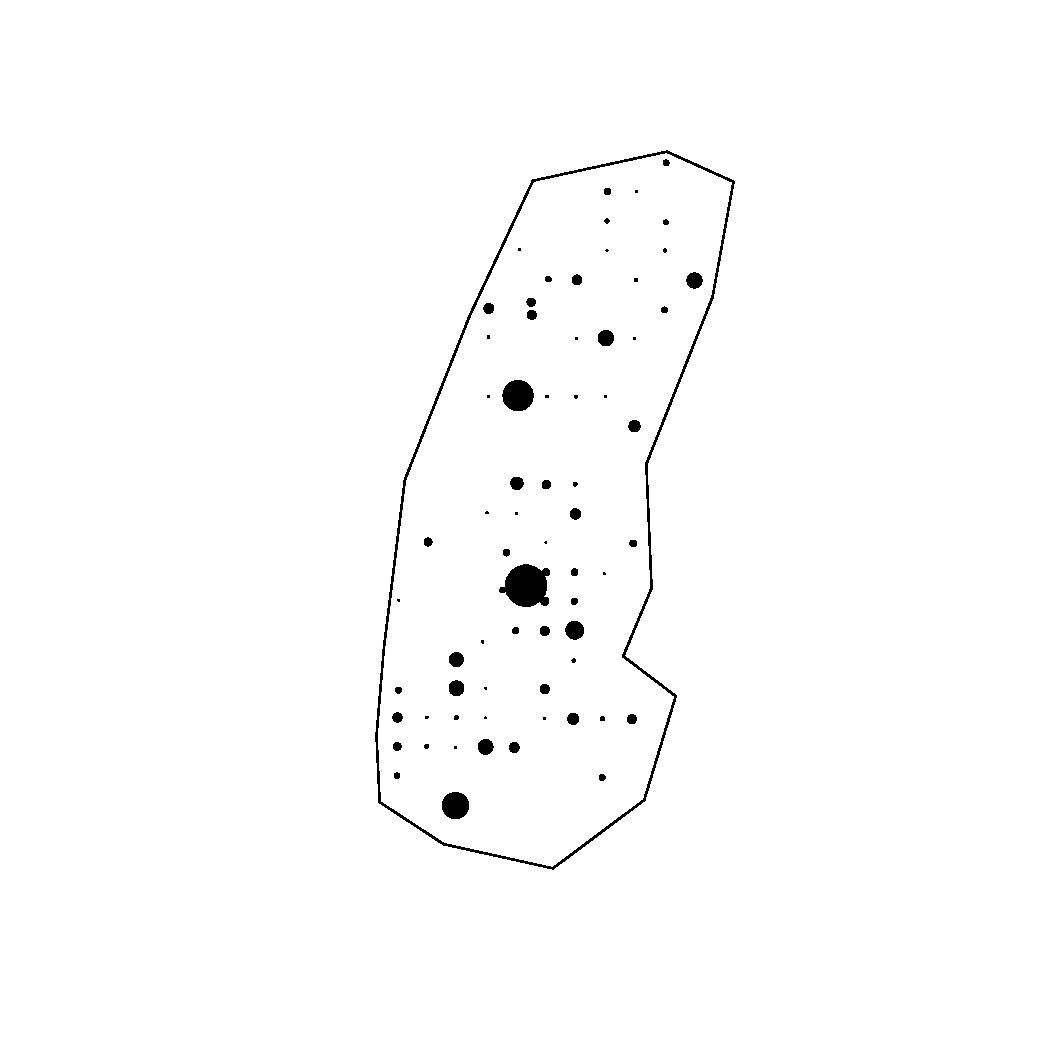
\includegraphics[width=.49\linewidth,scale=1]{Figures/CarteVolBMS-1} 

}

}
\subfloat[sup à 30 cm\label{fig:CarteVolBMS2}]{

{\centering 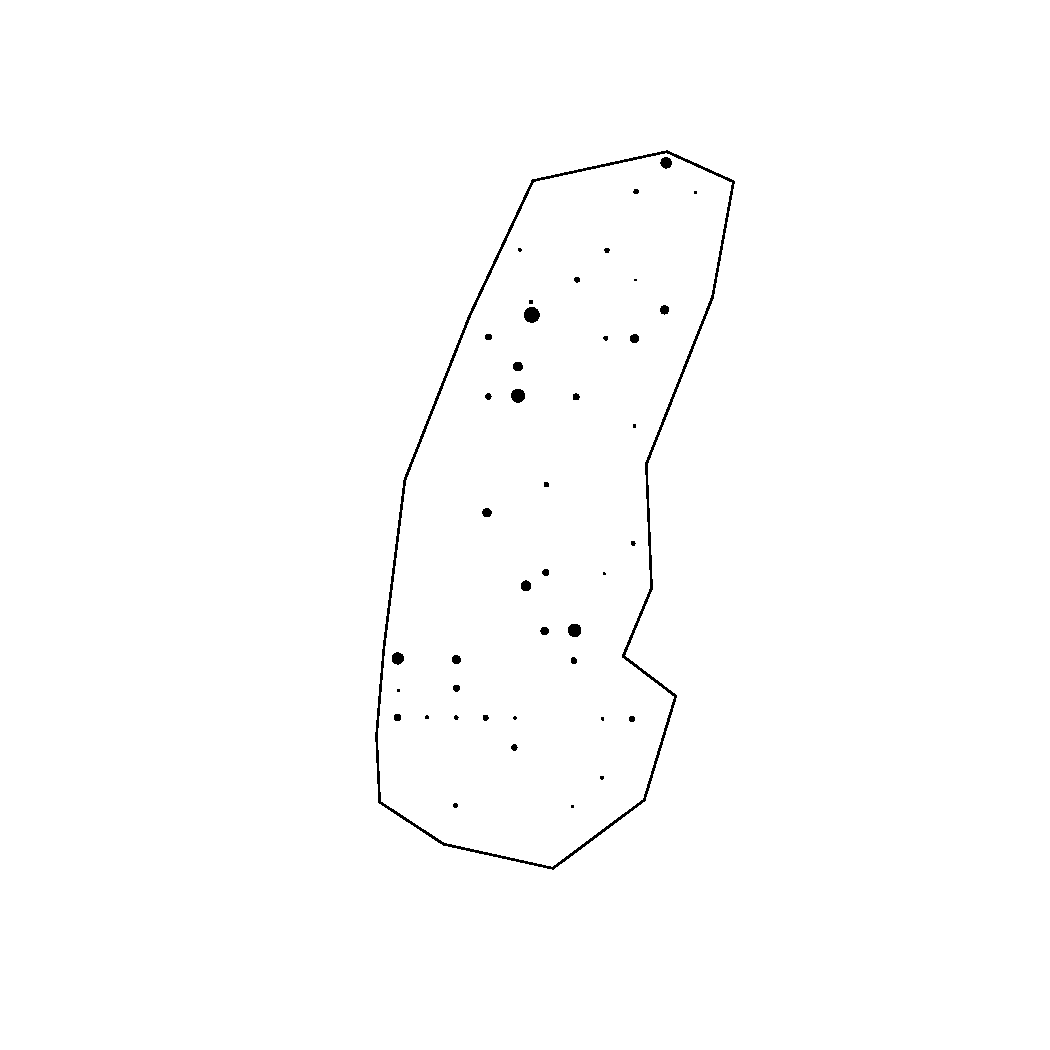
\includegraphics[width=.49\linewidth,scale=1]{Figures/CarteVolBMS-2} 

}

}\caption[Cartographie du volume de bois mort au sol]{Cartographie du volume de bois mort au sol.\label{fig:CarteVolBMS}}
\end{figure}


\end{knitrout}

\begin{knitrout}
\definecolor{shadecolor}{rgb}{0.969, 0.969, 0.969}\color{fgcolor}\begin{figure}[H]
\subfloat[inf à 30 cm\label{fig:CarteVolBMP1}]{

{\centering 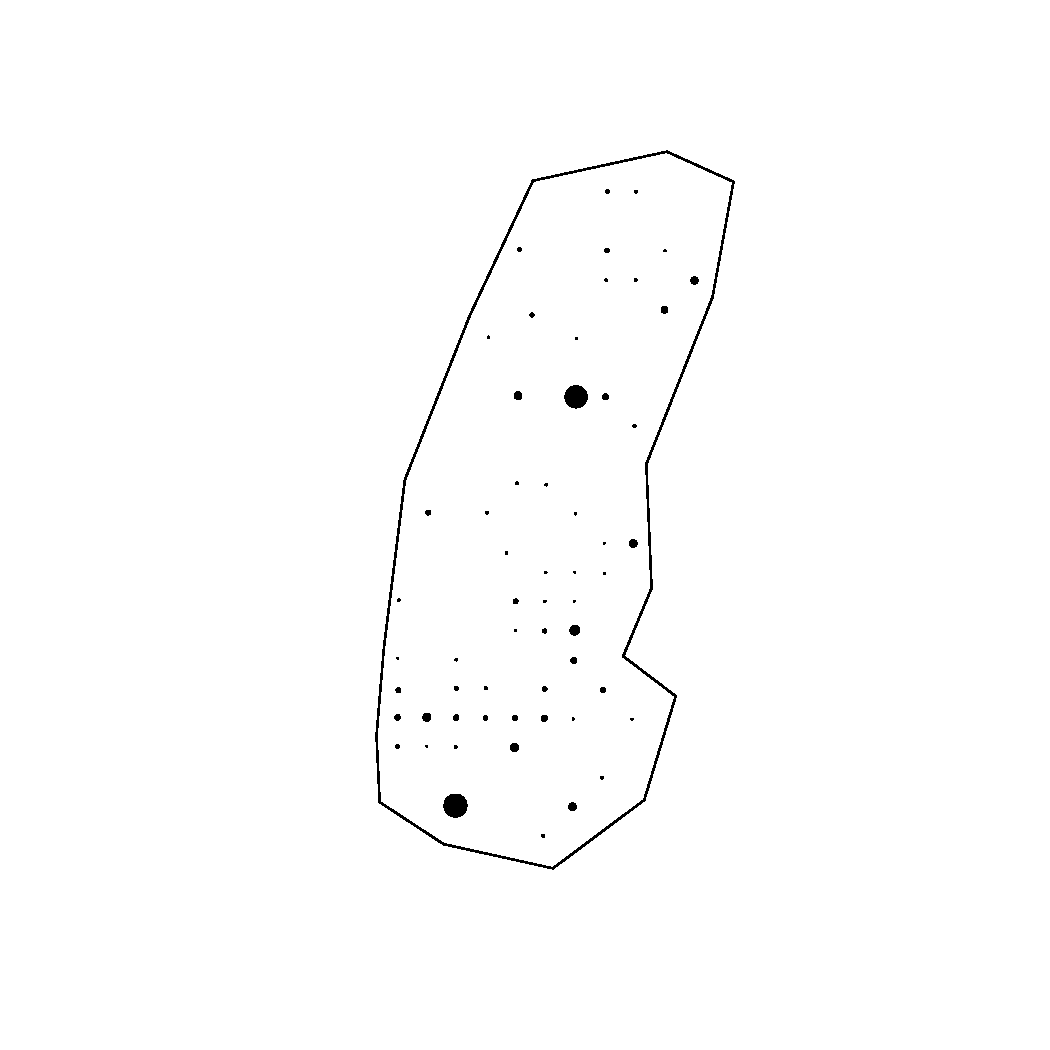
\includegraphics[width=.49\linewidth,scale=1]{Figures/CarteVolBMP-1} 

}

}
\subfloat[sup à 30 cm\label{fig:CarteVolBMP2}]{

{\centering 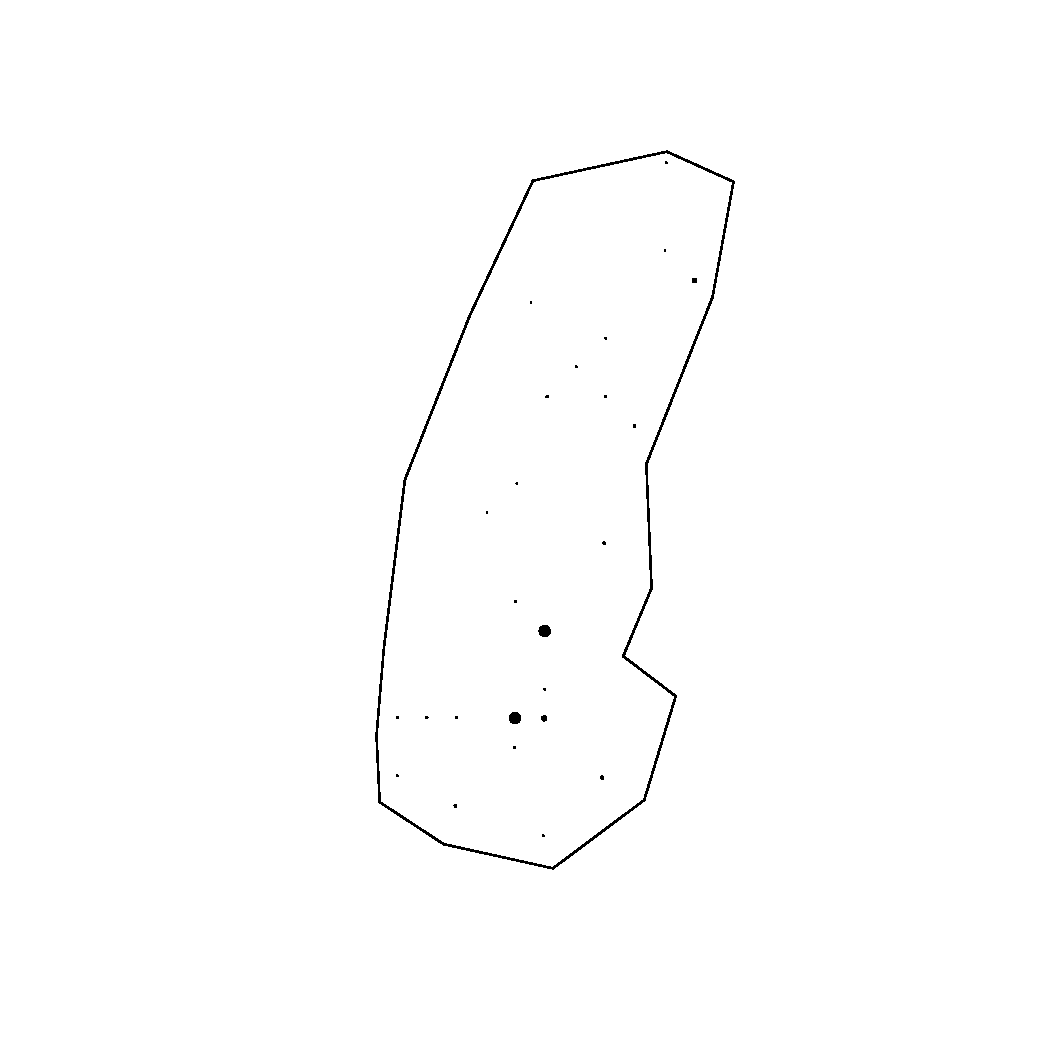
\includegraphics[width=.49\linewidth,scale=1]{Figures/CarteVolBMP-2} 

}

}\caption[Cartographie du volume de bois mort sur pied]{Cartographie du volume de bois mort sur pied.\label{fig:CarteVolBMP}}
\end{figure}


\end{knitrout}



\chapter{Bois vivant}

\section {Histogrammes}
La figure \ref{fig:Classe} permet de visualiser les histogrammes en volume et en nombre de tiges par classe de diamètre.

\begin{knitrout}\footnotesize
\definecolor{shadecolor}{rgb}{0.969, 0.969, 0.969}\color{fgcolor}\begin{figure}[h]
\subfloat[En volume\label{fig:Classe1}]{

{\centering 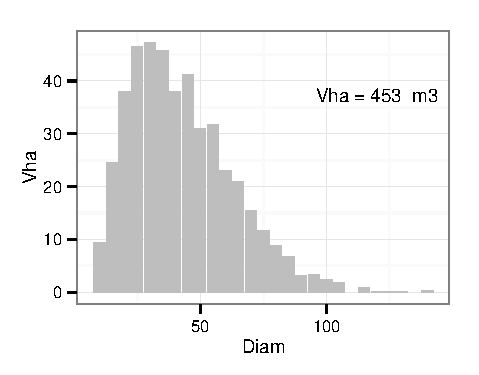
\includegraphics[width=.49\linewidth,scale=1]{Figures/Classe-1} 

}

}
\subfloat[En nombre de tiges\label{fig:Classe2}]{

{\centering 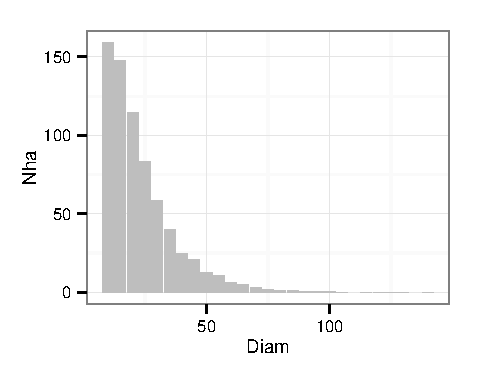
\includegraphics[width=.49\linewidth,scale=1]{Figures/Classe-2} 

}

}\caption[Répartition du matériel vivant sur pied par classe de diamètre]{Répartition du matériel vivant sur pied par classe de diamètre.\label{fig:Classe}}
\end{figure}


\end{knitrout}

\section{Composition}

\subsection{Biodiversité}


Le dispositif possède au total 12 espèces sous forme de semis, de brins de taillis ou d'arbres de franc-pied. La figure \ref{fig:CompoGlobal} donne une image de l'importance des essences dans chacun des stades de vie de l'arbre. Elle fournit la composition en pourcentage du volume pour les arbres (diamètre supérieur à 7,5cm) du recouvrement pour les semis inférieur à 50 cm de haut, et du nombre de tiges pour les différentes classes (class1, class2, class3) de semis de hauteur supérieure à 50 cm. Lorsqu'une classe de semis est absente, elle n'est pas représentée. \\
Cette figure \ref{fig:CompoGlobal} est une représentation visuelle de l'indice de biodiversité de Shannon.

\begin{knitrout}
\definecolor{shadecolor}{rgb}{0.969, 0.969, 0.969}\color{fgcolor}\begin{figure}[]


{\centering 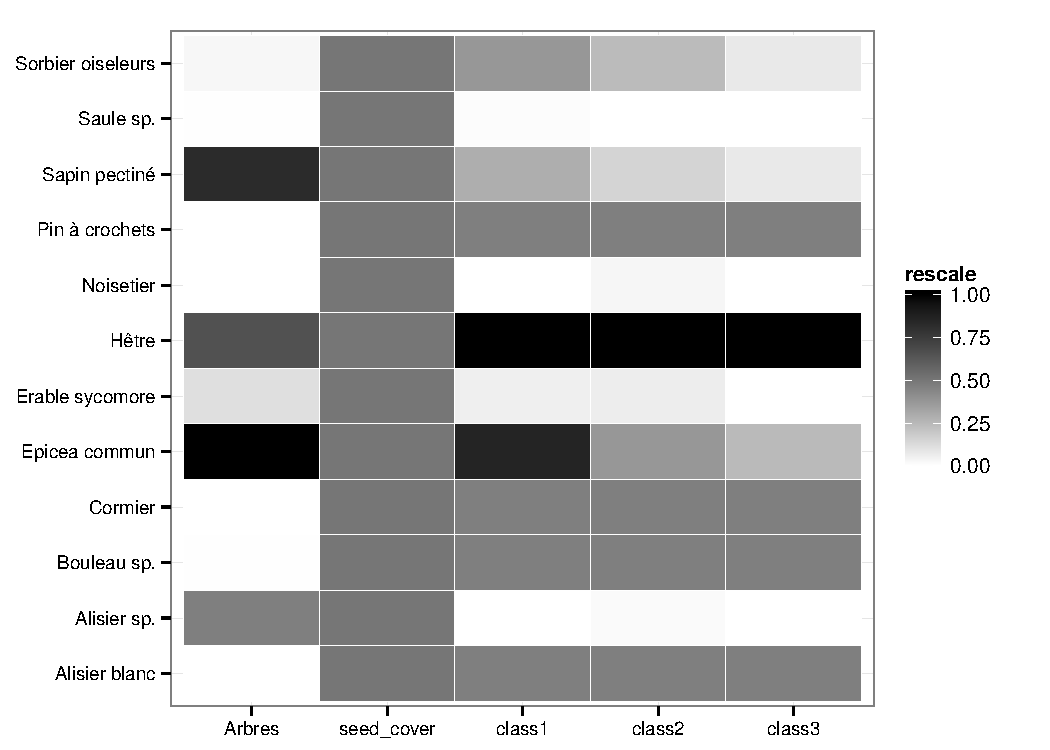
\includegraphics[width=\maxwidth]{Figures/CompoGlobal-1} 

}

\caption[Importance des essences selon les différents stades de vie de l'arbre]{Importance des essences selon les différents stades de vie de l'arbre.\label{fig:CompoGlobal}}
\end{figure}


\end{knitrout}


\subsection{Importance relative}
La figure \ref{fig:Compo} illustre l'importance relative des différentes essences. Elle est constituée de 2 graphiques : \\
- Celui de gauche fournit l'importance des différentes essences en nombre de tige (Nha), volume (Vha). \\
- Celui de droite fournit la répartition en nombre de tiges par classes de diamètre des différentes essences.

\begin{knitrout}
\definecolor{shadecolor}{rgb}{0.969, 0.969, 0.969}\color{fgcolor}\begin{figure}[htdp]


{\centering 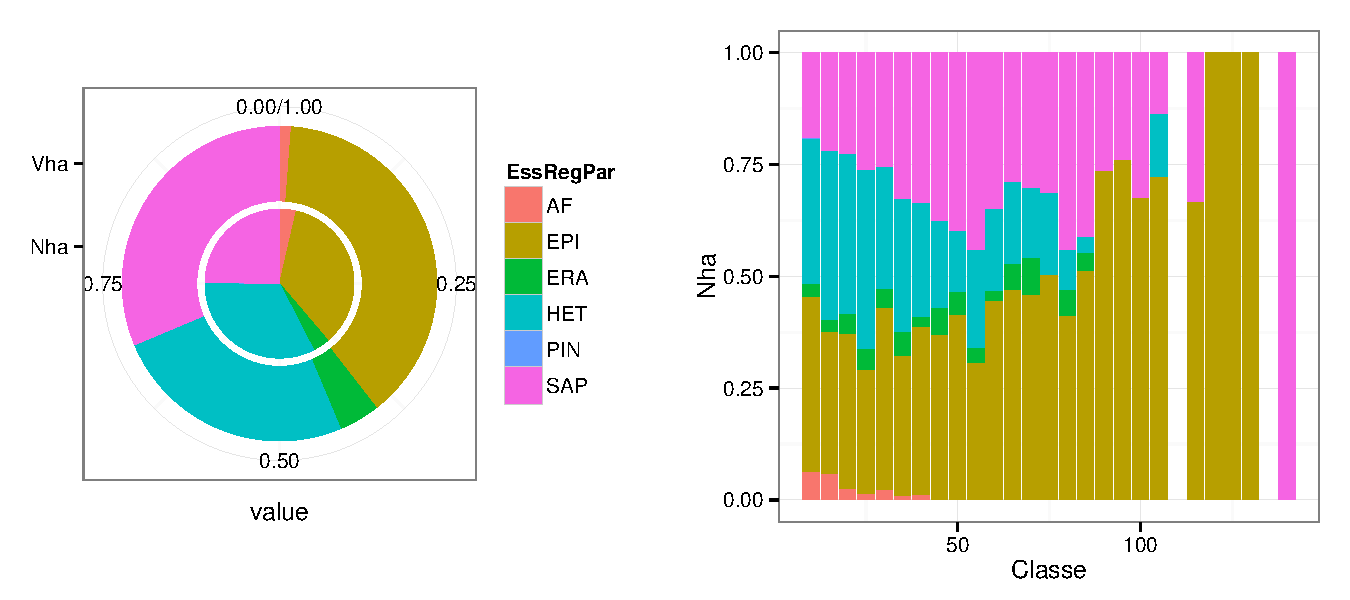
\includegraphics[width=\maxwidth]{Figures/Compo-1} 

}

\caption[Importance relative des différentes essences]{Importance relative des différentes essences.\label{fig:Compo}}
\end{figure}


\end{knitrout}


\subsection{Composition et structure}
La figure \ref{fig:Compo} illustre
\begin{knitrout}
\definecolor{shadecolor}{rgb}{0.969, 0.969, 0.969}\color{fgcolor}\begin{figure}[h]


{\centering 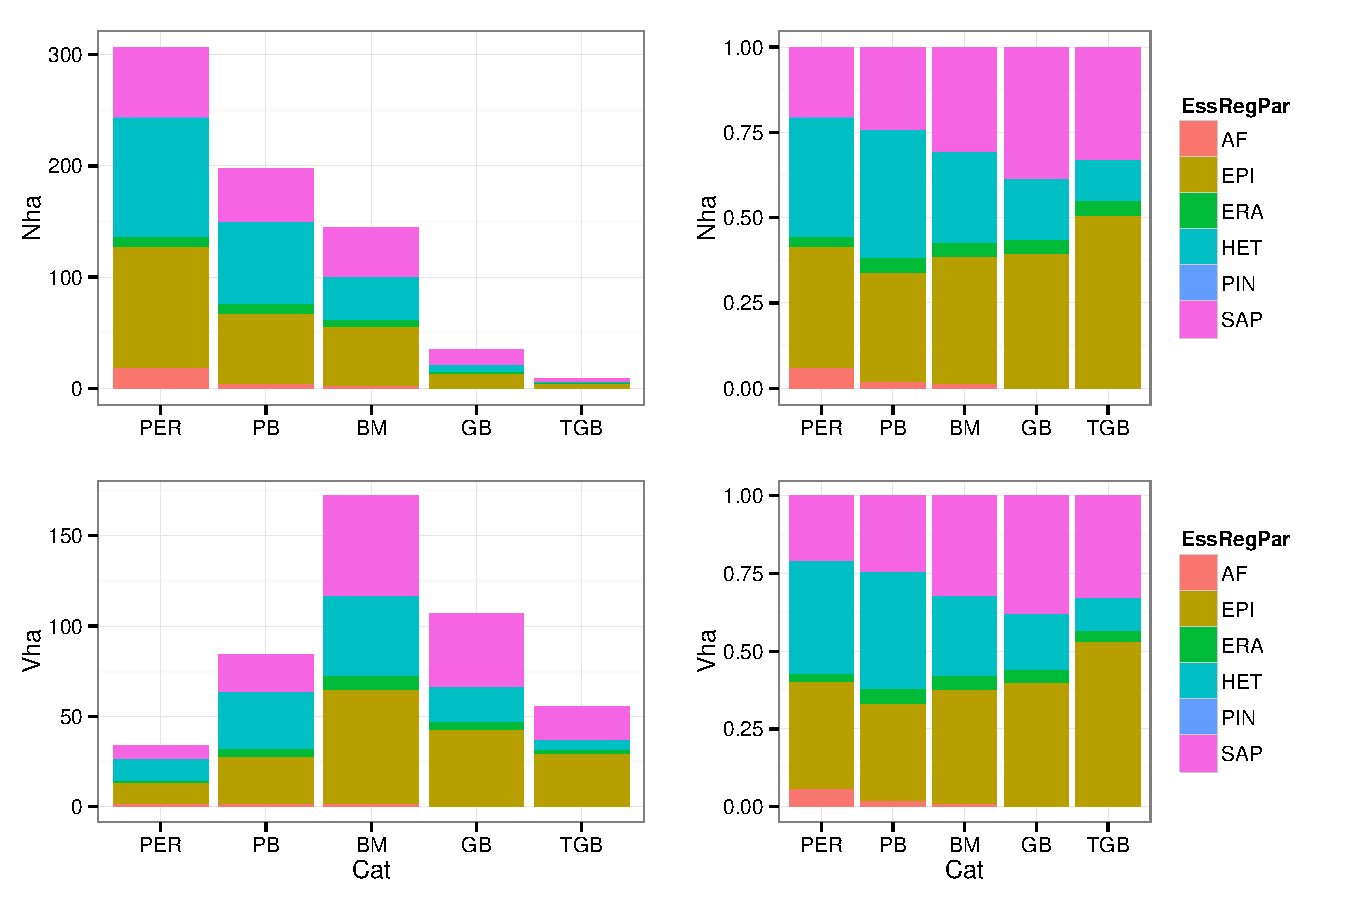
\includegraphics[width=\maxwidth]{Figures/CompoNG-1} 

}

\caption[Composition en essence en nombre de tige et en surface terrière, de manière absolue ou relative]{Composition en essence en nombre de tige et en surface terrière, de manière absolue ou relative.\label{fig:CompoNG}}
\end{figure}


\end{knitrout}



\chapter{Bois mort}

\section{Répartition par stade de décomposition}

La figure \ref{fig:BMStades} fournit l'importance du bois mort exprimée en volume, par grande catégorie de dimension et par stade de décomposition.

\begin{knitrout}
\definecolor{shadecolor}{rgb}{0.969, 0.969, 0.969}\color{fgcolor}\begin{figure}[H]
\subfloat[Stade de dureté\label{fig:BMStades1}]{

{\centering 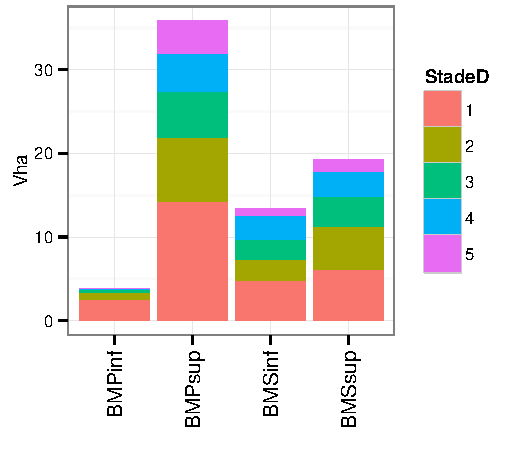
\includegraphics[width=\maxwidth]{Figures/BMStades-1} 

}

}
\subfloat[Stade d'écorce\label{fig:BMStades2}]{

{\centering 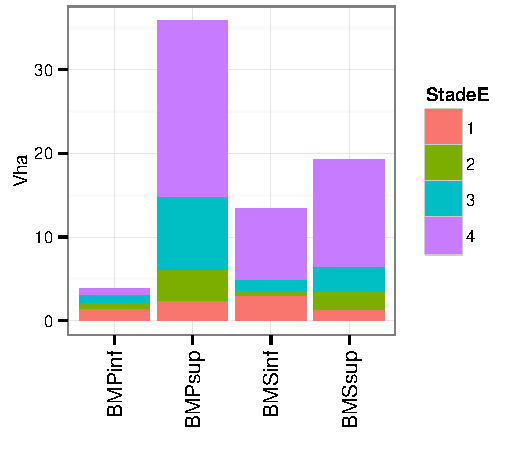
\includegraphics[width=\maxwidth]{Figures/BMStades-2} 

}

}\caption[Importance du bois mort par stades de décomposition]{Importance du bois mort par stades de décomposition.\label{fig:BMStades}}
\end{figure}


\end{knitrout}

\section{Répartition du bois mort sur pied par type}

\begin{knitrout}\footnotesize
\definecolor{shadecolor}{rgb}{0.969, 0.969, 0.969}\color{fgcolor}\begin{figure}[H]


{\centering 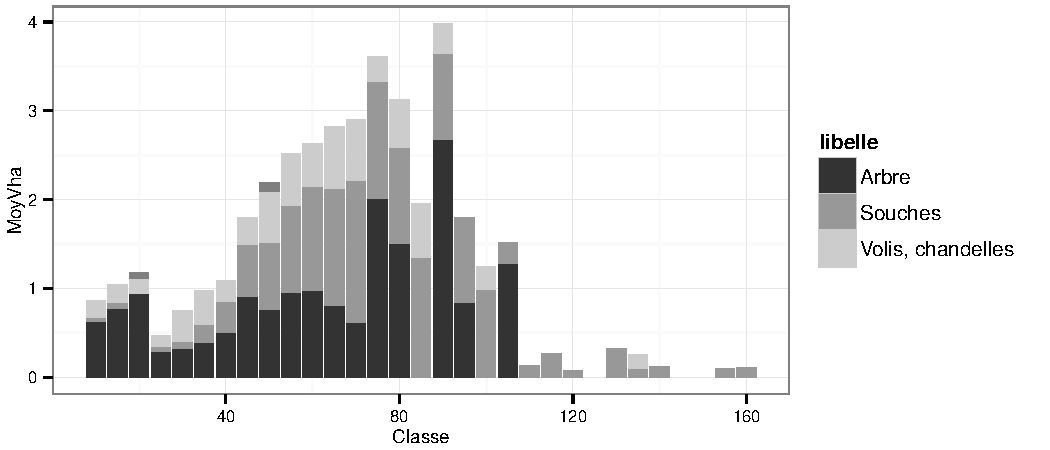
\includegraphics[width=\maxwidth]{Figures/BMPtypo-1} 

}

\caption[Répartition du bois mort sur pied par type]{Répartition du bois mort sur pied par type\label{fig:BMPtypo}}
\end{figure}


\end{knitrout}



\section{Ratio bois mort sur bois vivant}

\subsection{Par classe de diamètre}
\begin{knitrout}\footnotesize
\definecolor{shadecolor}{rgb}{0.969, 0.969, 0.969}\color{fgcolor}\begin{figure}[H]


{\centering 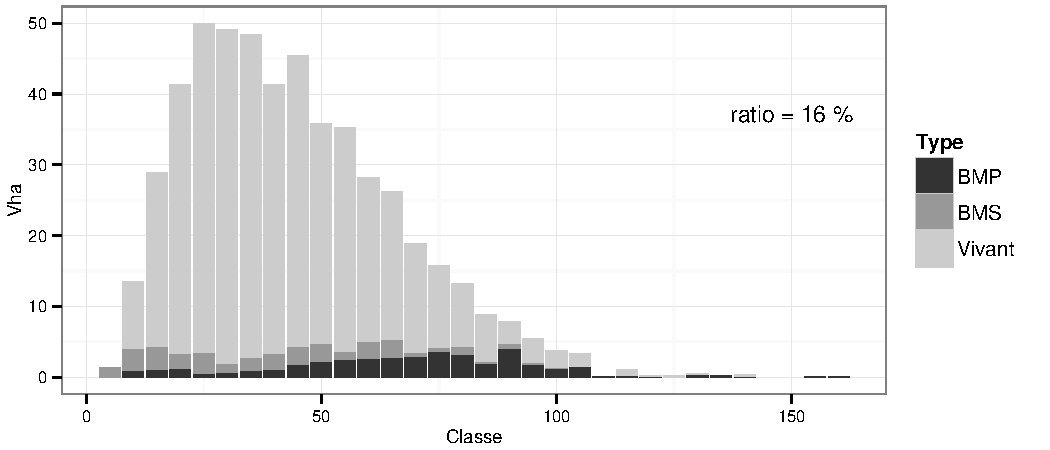
\includegraphics[width=\maxwidth]{Figures/Ratio-1} 

}

\caption[Importance relative du bois mort par classes de diamètre]{Importance relative du bois mort par classes de diamètre.\label{fig:Ratio}}
\end{figure}


\end{knitrout}

\subsection{Répartition du volume}

\subsubsection{Total}
\begin{knitrout}
\definecolor{shadecolor}{rgb}{0.969, 0.969, 0.969}\color{fgcolor}\begin{figure}[h]


{\centering 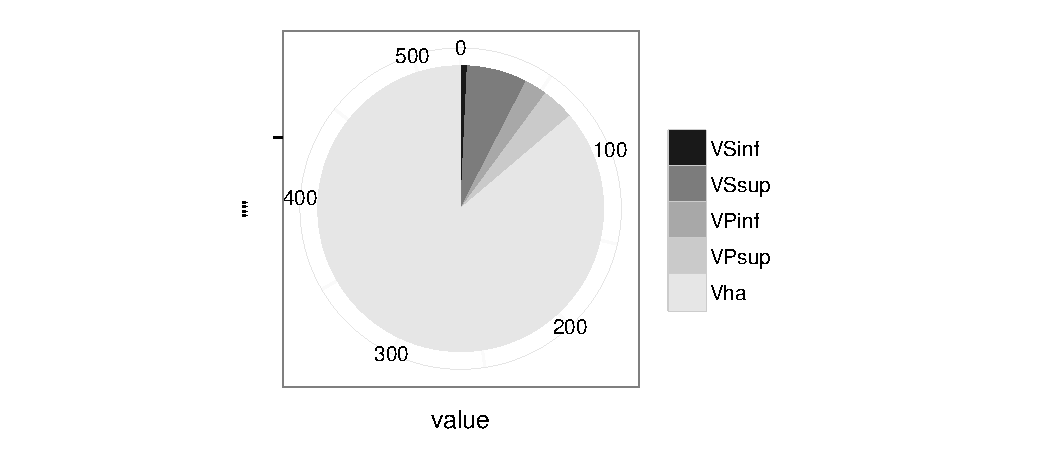
\includegraphics[width=\maxwidth]{Figures/RepVol-1} 

}

\caption[Répartition du volume]{Répartition du volume\label{fig:RepVol}}
\end{figure}


\end{knitrout}


\chapter{Codes écologiques}

\section{microhabitats}
Hist : N  ou N arbres porteurs microhabitats (sous ensemble position)

Hist : N microhabitats ou N arbres porteurs microhabitats (vitalité)

Graph : Note écologique/essence/cat diamètre

Graph : camemberts essences / hist (Ncodes/ha/essence) /codes regroupés


\section{État de conservation}

Tableau essences autochtones / allochtones


\chapter{Renouvellement}

\section{Régénération}

\subsection{Par stade de développement}
\begin{knitrout}\footnotesize
\definecolor{shadecolor}{rgb}{0.969, 0.969, 0.969}\color{fgcolor}\begin{figure}[h]


{\centering 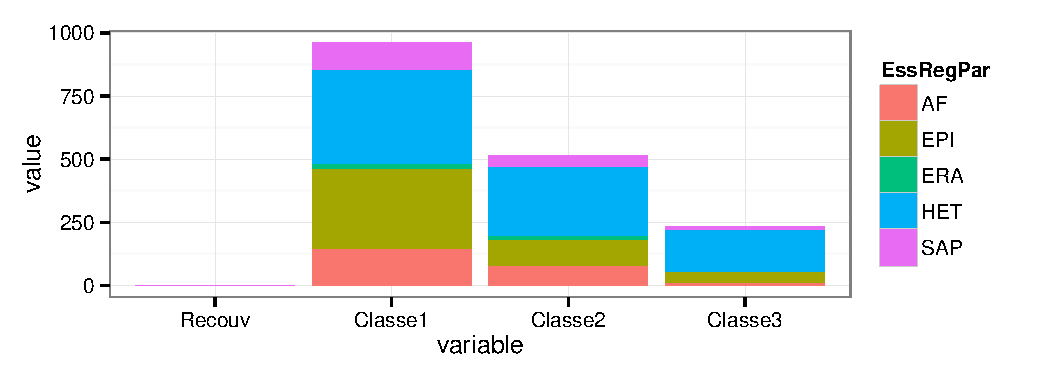
\includegraphics[width=\maxwidth]{Figures/Rege1-1} 

}

\caption[Régénération par stade de développement]{Régénération par stade de développement.\label{fig:Rege1}}
\end{figure}


\end{knitrout}

\subsection{Abroutissement}
\begin{knitrout}\footnotesize
\definecolor{shadecolor}{rgb}{0.969, 0.969, 0.969}\color{fgcolor}\begin{figure}[h]


{\centering 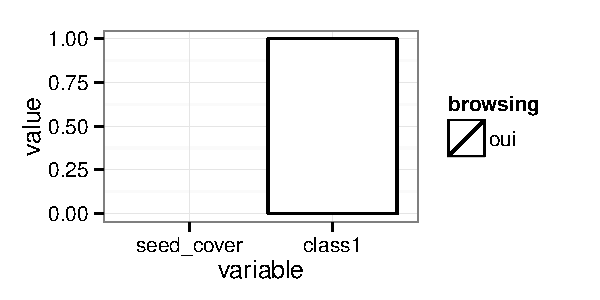
\includegraphics[width=\maxwidth]{Figures/Abroutissement-1} 

}

\caption[Abroutissement]{Abroutissement.\label{fig:Abroutissement}}
\end{figure}


\end{knitrout}




\chapter{Annexes}

\section{Analyse de l'échantillon}
\subsection{Adéquation échantillon/protocole}
\begin{knitrout}
\definecolor{shadecolor}{rgb}{0.969, 0.969, 0.969}\color{fgcolor}\begin{figure}[h]


{\centering 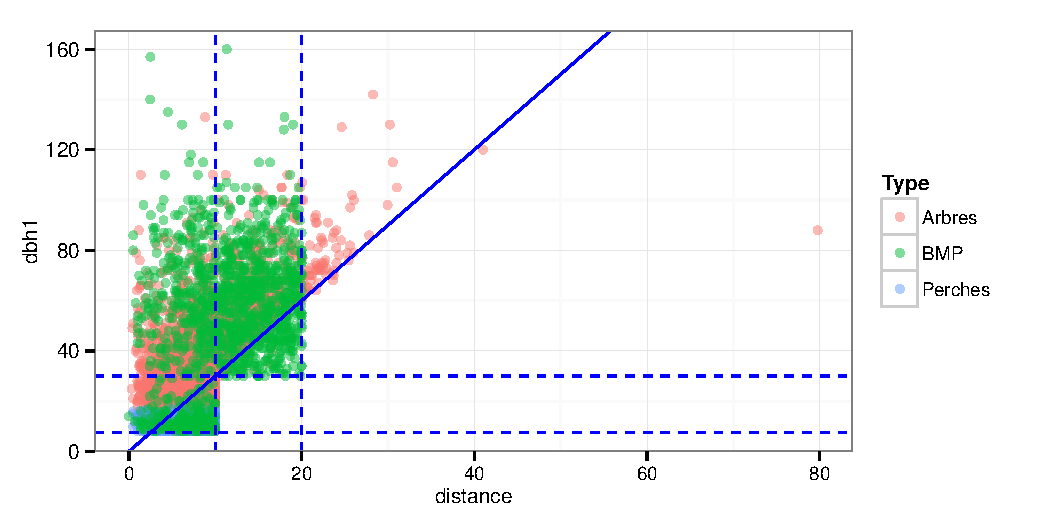
\includegraphics[width=\maxwidth]{Figures/DiamDist-1} 

}

\caption[Vérification de l'échantillon]{Vérification de l'échantillon.\label{fig:DiamDist}}
\end{figure}


\end{knitrout}

\subsection{Richesse en espèces ligneuses}
\begin{knitrout}
\definecolor{shadecolor}{rgb}{0.969, 0.969, 0.969}\color{fgcolor}\begin{figure}[h]


{\centering 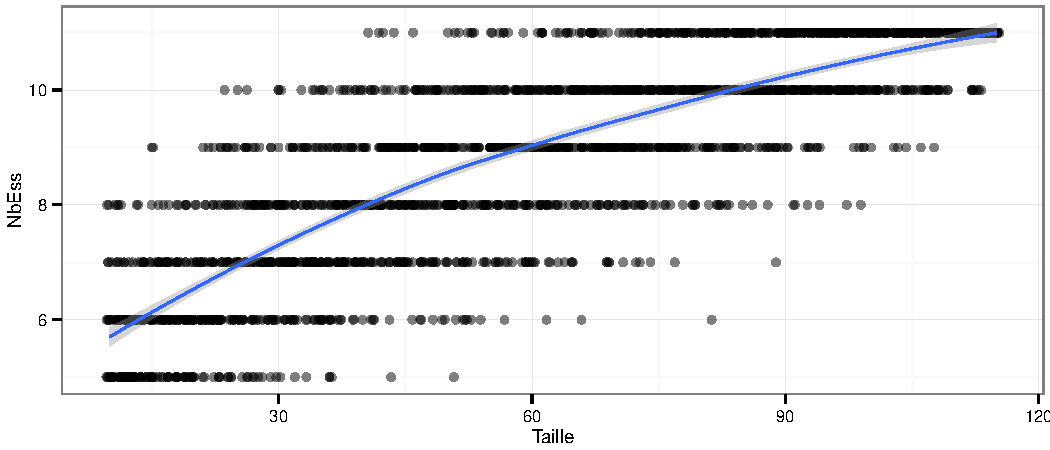
\includegraphics[width=\maxwidth]{Figures/Bootstrap-1} 

}

\caption[Qualité de l'estimation de la richesse en espèce en fonction du nombre de placette]{Qualité de l'estimation de la richesse en espèce en fonction du nombre de placette.\label{fig:Bootstrap}}
\end{figure}


\end{knitrout}



\section{Tarifs de cubage retenus par l'opérateur}
Le tableau \ref{TarifsOp} liste les tarifs de cubage par essence retenus par le gestionnaire.
% latex table generated in R 3.1.2 by xtable 1.7-4 package
% Mon Nov 24 09:52:19 2014
\begin{table}[ht]
\centering
{\footnotesize
\begin{tabular}{llr}
  \hline
Essence & Type de tarif & Numéro \\ 
  \hline
Alisier blanc & schl & 12 \\ 
  Bouleau blanc & schl & 12 \\ 
  Cormier & schl & 12 \\ 
  Epicea commun & schl & 12 \\ 
  Erable sycomore & schl & 12 \\ 
  Hêtre & schl & 12 \\ 
  Noisetier & schl & 12 \\ 
  Orme sp. & schl & 12 \\ 
  Pin à crochets & schl & 12 \\ 
  Sapin pectiné & schl & 12 \\ 
  Saule sp. & schl & 12 \\ 
  Sorbier oiseleurs & schl & 12 \\ 
   \hline
\end{tabular}
}
\caption{Tarifs de cubage retenus par le gestionnaire.} 
\label{TarifsOp}
\end{table}


\subsection{Tarifs de cubage volume géométrique bois fort tige}
Le tableau \ref{TarifsIFN} liste les tarifs de cubage par essence bois fort tige obtenus à partir de la base de données de l'IFN.



\section{Plans de localisation des arbres}
Ils sont situés dans un document annexe.
%
% <<PlanArbres, echo=FALSE, fig.height=9, fig.show='asis', fig.cap="Plan de localisation des arbres par placettes">>=
% pas <- 4
% Groupe <- unique(c(seq(1, NbPlac, by = pas), NbPlac))
% tab <- subset(Arbres, select=c("essence","plot","X","Y","dbh1"))
% tab <- merge(tab,psdrf_essence[,c("id","libelle")], by.x="essence", by.y="id", all.x=T)
%
% for (i in 2:length(Groupe)) {
%   j = Groupe[i-1]
%   m = ifelse(i==length(Groupe),max(Groupe),Groupe[i]-1)
%   ArbresEnTour <- subset(tab, plot %in% PlacEnTour$id[j:m])
%   ArbresEnTour <- merge(ArbresEnTour, psdrf_plot[,c("id","num")], by.x="plot", by.y="id", all.x=T)
%   p <- ggplot(ArbresEnTour, aes(x=X, y=Y, colour=libelle, size=dbh1)) + theme_bw( ) +
%     scale_x_continuous(limits = c(-25, 25)) + scale_y_continuous(limits = c(-25, 25)) +
%     coord_equal(ratio=1)
%   print(p + geom_point() + scale_size(range = c(2, 10)) + facet_wrap(~ num, nrow=2, ncol=2) +
%           theme(legend.text = element_text(size = 6), plot.margin = unit(c(0.1,0.1,0,0), "cm"))
%         )
% }
% @
%


\end{document}
